\documentclass[twoside]{book}

% Packages required by doxygen
\usepackage{fixltx2e}
\usepackage{calc}
\usepackage{doxygen}
\usepackage[export]{adjustbox} % also loads graphicx
\usepackage{graphicx}
\usepackage[utf8]{inputenc}
\usepackage{makeidx}
\usepackage{multicol}
\usepackage{multirow}
\PassOptionsToPackage{warn}{textcomp}
\usepackage{textcomp}
\usepackage[nointegrals]{wasysym}
\usepackage[table]{xcolor}

% Font selection
\usepackage[T1]{fontenc}
\usepackage[scaled=.90]{helvet}
\usepackage{courier}
\usepackage{amssymb}
\usepackage{sectsty}
\renewcommand{\familydefault}{\sfdefault}
\allsectionsfont{%
  \fontseries{bc}\selectfont%
  \color{darkgray}%
}
\renewcommand{\DoxyLabelFont}{%
  \fontseries{bc}\selectfont%
  \color{darkgray}%
}
\newcommand{\+}{\discretionary{\mbox{\scriptsize$\hookleftarrow$}}{}{}}

% Page & text layout
\usepackage{geometry}
\geometry{%
  a4paper,%
  top=2.5cm,%
  bottom=2.5cm,%
  left=2.5cm,%
  right=2.5cm%
}
\tolerance=750
\hfuzz=15pt
\hbadness=750
\setlength{\emergencystretch}{15pt}
\setlength{\parindent}{0cm}
\setlength{\parskip}{3ex plus 2ex minus 2ex}
\makeatletter
\renewcommand{\paragraph}{%
  \@startsection{paragraph}{4}{0ex}{-1.0ex}{1.0ex}{%
    \normalfont\normalsize\bfseries\SS@parafont%
  }%
}
\renewcommand{\subparagraph}{%
  \@startsection{subparagraph}{5}{0ex}{-1.0ex}{1.0ex}{%
    \normalfont\normalsize\bfseries\SS@subparafont%
  }%
}
\makeatother

% Headers & footers
\usepackage{fancyhdr}
\pagestyle{fancyplain}
\fancyhead[LE]{\fancyplain{}{\bfseries\thepage}}
\fancyhead[CE]{\fancyplain{}{}}
\fancyhead[RE]{\fancyplain{}{\bfseries\leftmark}}
\fancyhead[LO]{\fancyplain{}{\bfseries\rightmark}}
\fancyhead[CO]{\fancyplain{}{}}
\fancyhead[RO]{\fancyplain{}{\bfseries\thepage}}
\fancyfoot[LE]{\fancyplain{}{}}
\fancyfoot[CE]{\fancyplain{}{}}
\fancyfoot[RE]{\fancyplain{}{\bfseries\scriptsize Generated by Doxygen }}
\fancyfoot[LO]{\fancyplain{}{\bfseries\scriptsize Generated by Doxygen }}
\fancyfoot[CO]{\fancyplain{}{}}
\fancyfoot[RO]{\fancyplain{}{}}
\renewcommand{\footrulewidth}{0.4pt}
\renewcommand{\chaptermark}[1]{%
  \markboth{#1}{}%
}
\renewcommand{\sectionmark}[1]{%
  \markright{\thesection\ #1}%
}

% Indices & bibliography
\usepackage{natbib}
\usepackage[titles]{tocloft}
\setcounter{tocdepth}{3}
\setcounter{secnumdepth}{5}
\makeindex

% Hyperlinks (required, but should be loaded last)
\usepackage{ifpdf}
\ifpdf
  \usepackage[pdftex,pagebackref=true]{hyperref}
\else
  \usepackage[ps2pdf,pagebackref=true]{hyperref}
\fi
\hypersetup{%
  colorlinks=true,%
  linkcolor=blue,%
  citecolor=blue,%
  unicode%
}

% Custom commands
\newcommand{\clearemptydoublepage}{%
  \newpage{\pagestyle{empty}\cleardoublepage}%
}

\usepackage{caption}
\captionsetup{labelsep=space,justification=centering,font={bf},singlelinecheck=off,skip=4pt,position=top}

%===== C O N T E N T S =====

\begin{document}

% Titlepage & ToC
\hypersetup{pageanchor=false,
             bookmarksnumbered=true,
             pdfencoding=unicode
            }
\pagenumbering{alph}
\begin{titlepage}
\vspace*{7cm}
\begin{center}%
{\Large Heisprosjekt }\\
\vspace*{1cm}
{\large Generated by Doxygen 1.8.13}\\
\end{center}
\end{titlepage}
\clearemptydoublepage
\pagenumbering{roman}
\tableofcontents
\clearemptydoublepage
\pagenumbering{arabic}
\hypersetup{pageanchor=true}

%--- Begin generated contents ---
\chapter{Data Structure Index}
\section{Data Structures}
Here are the data structures with brief descriptions\+:\begin{DoxyCompactList}
\item\contentsline{section}{\hyperlink{structState}{State} \\*A struct with members that hold information about the elevators state }{\pageref{structState}}{}
\end{DoxyCompactList}

\chapter{File Index}
\section{File List}
Here is a list of all documented files with brief descriptions\+:\begin{DoxyCompactList}
\item\contentsline{section}{source/\hyperlink{hardware_8h}{hardware.\+h} \\*Driver for the elevator hardware }{\pageref{hardware_8h}}{}
\item\contentsline{section}{source/{\bfseries main.\+c} }{\pageref{main_8c}}{}
\item\contentsline{section}{source/\hyperlink{state_8h}{state.\+h} \\*States for the finite state machine }{\pageref{state_8h}}{}
\item\contentsline{section}{source/{\bfseries utilities.\+c} }{\pageref{utilities_8c}}{}
\item\contentsline{section}{source/\hyperlink{utilities_8h}{utilities.\+h} \\*Utility-\/functions that is used to make decisions regarding the initialization and handling of the fsm, as well as the high level logic of the hardware }{\pageref{utilities_8h}}{}
\item\contentsline{section}{source/driver/\hyperlink{channels_8h}{channels.\+h} \\*Channel definitions for elevator control using Lib\+Comedi 2006, Martin Korsgaard }{\pageref{channels_8h}}{}
\item\contentsline{section}{source/driver/{\bfseries hardware\+\_\+sal.\+c} }{\pageref{hardware__sal_8c}}{}
\item\contentsline{section}{source/driver/{\bfseries hardware\+\_\+sim.\+c} }{\pageref{hardware__sim_8c}}{}
\item\contentsline{section}{source/driver/{\bfseries io.\+c} }{\pageref{io_8c}}{}
\item\contentsline{section}{source/driver/\hyperlink{io_8h}{io.\+h} \\*Wrapper for lib\+Comedi I/O. These functions provide and interface to lib\+Comedi limited to use in the real time lab. 2006, Martin Korsgaard }{\pageref{io_8h}}{}
\end{DoxyCompactList}

\chapter{Data Structure Documentation}
\hypertarget{structState}{}\section{State Struct Reference}
\label{structState}\index{State@{State}}


A struct with members that hold information about the elevators state.  




{\ttfamily \#include $<$state.\+h$>$}

\subsection*{Data Fields}
\begin{DoxyCompactItemize}
\item 
\mbox{\Hypertarget{structState_a881e39b29ca021715cbb5f5a472c140f}\label{structState_a881e39b29ca021715cbb5f5a472c140f}} 
int {\bfseries fsm\+\_\+floor}
\item 
\mbox{\Hypertarget{structState_af805fd2224548bc74d5cb977da399b1c}\label{structState_af805fd2224548bc74d5cb977da399b1c}} 
int {\bfseries fsm\+\_\+stop}
\item 
\mbox{\Hypertarget{structState_aa1944221a61f699959e2dd2fb29537b1}\label{structState_aa1944221a61f699959e2dd2fb29537b1}} 
int {\bfseries fsm\+\_\+door}
\item 
\mbox{\Hypertarget{structState_a80de292fc4b9c7f578c61102b5ef6acc}\label{structState_a80de292fc4b9c7f578c61102b5ef6acc}} 
int {\bfseries fsm\+\_\+direction}
\item 
\mbox{\Hypertarget{structState_a486ebfe1ed84af6f4a04ac0c498d8fd9}\label{structState_a486ebfe1ed84af6f4a04ac0c498d8fd9}} 
int {\bfseries fsm\+\_\+orders} \mbox{[}H\+A\+R\+D\+W\+A\+R\+E\+\_\+\+N\+U\+M\+B\+E\+R\+\_\+\+O\+F\+\_\+\+F\+L\+O\+O\+RS\mbox{]}\mbox{[}3\mbox{]}
\item 
\mbox{\Hypertarget{structState_a81de86f445c82ce699a6250961dcffce}\label{structState_a81de86f445c82ce699a6250961dcffce}} 
int {\bfseries fsm\+\_\+ignore\+All\+Ordes}
\item 
\mbox{\Hypertarget{structState_a88bfd697dae6255ef2164c2025073a5b}\label{structState_a88bfd697dae6255ef2164c2025073a5b}} 
clock\+\_\+t {\bfseries timer\+\_\+start\+Time}
\item 
\mbox{\Hypertarget{structState_aded80ff67ae02afeebddbc45dd905160}\label{structState_aded80ff67ae02afeebddbc45dd905160}} 
clock\+\_\+t {\bfseries timer\+\_\+waiting\+Time}
\end{DoxyCompactItemize}


\subsection{Detailed Description}
A struct with members that hold information about the elevators state. 

fsm\+\_\+floor is the last floor of the elevator, form 0 to 3

fsm\+\_\+stop is true when in stop-\/mode and false if not

fsm\+\_\+door is true when the door is open, and false when closed

fsm\+\_\+direction is the current direction of the elevator; 1 when it is going down and 0 when going up

fsm\+\_\+orders is the orderbook; a matrix that keeps track of the orders, so a 1 indicates an unattended order, and a 0 means no orders. The first column indicates the down-\/order buttons outside the elevator, the second column indicates the up-\/order buttons outside the elevator and the third column is the order buttons inside the elevator. Further indicates the first row the first floor, and so on to the last row, which indicates the top floor.

fsm\+\_\+ignore\+All\+Ordes When active, the elevator ignores all orders pending the arrival at the first floor Reset after arrival at the first floor

timer\+\_\+start\+Time is the time when the door timer starts

timer\+\_\+waiting\+Time is the door waiting-\//countdowntime 

Definition at line 37 of file state.\+h.



The documentation for this struct was generated from the following file\+:\begin{DoxyCompactItemize}
\item 
source/\hyperlink{state_8h}{state.\+h}\end{DoxyCompactItemize}

\chapter{File Documentation}
\hypertarget{channels_8h}{}\section{source/driver/channels.h File Reference}
\label{channels_8h}\index{source/driver/channels.\+h@{source/driver/channels.\+h}}


Channel definitions for elevator control using Lib\+Comedi 2006, Martin Korsgaard.  


This graph shows which files directly or indirectly include this file\+:\nopagebreak
\begin{figure}[H]
\begin{center}
\leavevmode
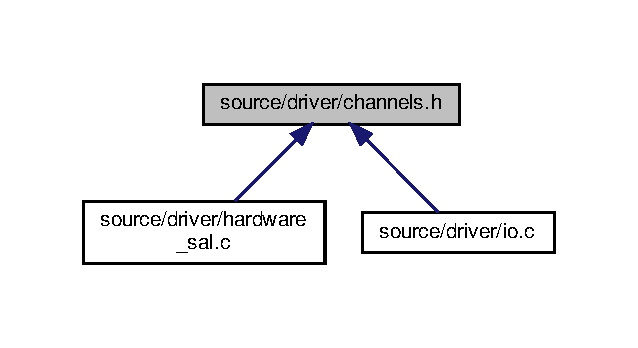
\includegraphics[width=306pt]{channels_8h__dep__incl}
\end{center}
\end{figure}
\subsection*{Macros}
\begin{DoxyCompactItemize}
\item 
\mbox{\Hypertarget{channels_8h_ad5a54f368997d8ae4f84a1e2fad533f4}\label{channels_8h_ad5a54f368997d8ae4f84a1e2fad533f4}} 
\#define {\bfseries P\+O\+R\+T4}~3
\item 
\mbox{\Hypertarget{channels_8h_a2409f02d98d288f64712887bd13b853e}\label{channels_8h_a2409f02d98d288f64712887bd13b853e}} 
\#define {\bfseries O\+B\+S\+T\+R\+U\+C\+T\+I\+ON}~(0x300+23)
\item 
\mbox{\Hypertarget{channels_8h_ae19b6bb2940d2fbe0a79852b070eeafd}\label{channels_8h_ae19b6bb2940d2fbe0a79852b070eeafd}} 
\#define {\bfseries S\+T\+OP}~(0x300+22)
\item 
\mbox{\Hypertarget{channels_8h_a1a22e01173ae543c7350d23af9099083}\label{channels_8h_a1a22e01173ae543c7350d23af9099083}} 
\#define {\bfseries B\+U\+T\+T\+O\+N\+\_\+\+C\+O\+M\+M\+A\+N\+D1}~(0x300+21)
\item 
\mbox{\Hypertarget{channels_8h_a8f3d02fddfb1ecd5227eca135f19ebd6}\label{channels_8h_a8f3d02fddfb1ecd5227eca135f19ebd6}} 
\#define {\bfseries B\+U\+T\+T\+O\+N\+\_\+\+C\+O\+M\+M\+A\+N\+D2}~(0x300+20)
\item 
\mbox{\Hypertarget{channels_8h_a82aab21b1b50d554effcf8b26576b388}\label{channels_8h_a82aab21b1b50d554effcf8b26576b388}} 
\#define {\bfseries B\+U\+T\+T\+O\+N\+\_\+\+C\+O\+M\+M\+A\+N\+D3}~(0x300+19)
\item 
\mbox{\Hypertarget{channels_8h_add9ae7df96dfd4ad569d3b703023187d}\label{channels_8h_add9ae7df96dfd4ad569d3b703023187d}} 
\#define {\bfseries B\+U\+T\+T\+O\+N\+\_\+\+C\+O\+M\+M\+A\+N\+D4}~(0x300+18)
\item 
\mbox{\Hypertarget{channels_8h_a7236f6ea90139248afabe014632c3cec}\label{channels_8h_a7236f6ea90139248afabe014632c3cec}} 
\#define {\bfseries B\+U\+T\+T\+O\+N\+\_\+\+U\+P1}~(0x300+17)
\item 
\mbox{\Hypertarget{channels_8h_a3a95d31cf2002937c921bbd85590bc7a}\label{channels_8h_a3a95d31cf2002937c921bbd85590bc7a}} 
\#define {\bfseries B\+U\+T\+T\+O\+N\+\_\+\+U\+P2}~(0x300+16)
\item 
\mbox{\Hypertarget{channels_8h_a83b698b796fa8d1625536439f28ea575}\label{channels_8h_a83b698b796fa8d1625536439f28ea575}} 
\#define {\bfseries P\+O\+R\+T1}~2
\item 
\mbox{\Hypertarget{channels_8h_a63a7b9d9d7c23325d4171292d596fa11}\label{channels_8h_a63a7b9d9d7c23325d4171292d596fa11}} 
\#define {\bfseries B\+U\+T\+T\+O\+N\+\_\+\+D\+O\+W\+N2}~(0x200+0)
\item 
\mbox{\Hypertarget{channels_8h_aa6b5917715e012cf21e3a89fb7c93e2d}\label{channels_8h_aa6b5917715e012cf21e3a89fb7c93e2d}} 
\#define {\bfseries B\+U\+T\+T\+O\+N\+\_\+\+U\+P3}~(0x200+1)
\item 
\mbox{\Hypertarget{channels_8h_ab423174da71ed0d6b083cd8d71f54617}\label{channels_8h_ab423174da71ed0d6b083cd8d71f54617}} 
\#define {\bfseries B\+U\+T\+T\+O\+N\+\_\+\+D\+O\+W\+N3}~(0x200+2)
\item 
\mbox{\Hypertarget{channels_8h_a7e1266fcb6843826718edec0222b1e49}\label{channels_8h_a7e1266fcb6843826718edec0222b1e49}} 
\#define {\bfseries B\+U\+T\+T\+O\+N\+\_\+\+D\+O\+W\+N4}~(0x200+3)
\item 
\mbox{\Hypertarget{channels_8h_a5ae95fe4e1273653467895d5e7c39377}\label{channels_8h_a5ae95fe4e1273653467895d5e7c39377}} 
\#define {\bfseries S\+E\+N\+S\+O\+R\+\_\+\+F\+L\+O\+O\+R1}~(0x200+4)
\item 
\mbox{\Hypertarget{channels_8h_ab9e1c393bf2c51d65ed0a132af8321d3}\label{channels_8h_ab9e1c393bf2c51d65ed0a132af8321d3}} 
\#define {\bfseries S\+E\+N\+S\+O\+R\+\_\+\+F\+L\+O\+O\+R2}~(0x200+5)
\item 
\mbox{\Hypertarget{channels_8h_a65904322d022513386fea3bcb9a8b524}\label{channels_8h_a65904322d022513386fea3bcb9a8b524}} 
\#define {\bfseries S\+E\+N\+S\+O\+R\+\_\+\+F\+L\+O\+O\+R3}~(0x200+6)
\item 
\mbox{\Hypertarget{channels_8h_a6a8d30abdce8780479ac7f0677200074}\label{channels_8h_a6a8d30abdce8780479ac7f0677200074}} 
\#define {\bfseries S\+E\+N\+S\+O\+R\+\_\+\+F\+L\+O\+O\+R4}~(0x200+7)
\item 
\mbox{\Hypertarget{channels_8h_ad906b7f6a811f1f02b5eb04cbe1bc89b}\label{channels_8h_ad906b7f6a811f1f02b5eb04cbe1bc89b}} 
\#define {\bfseries P\+O\+R\+T3}~3
\item 
\mbox{\Hypertarget{channels_8h_aaa316c7fc13ca7b9b4229af3f9832a7d}\label{channels_8h_aaa316c7fc13ca7b9b4229af3f9832a7d}} 
\#define {\bfseries M\+O\+T\+O\+R\+D\+IR}~(0x300+15)
\item 
\mbox{\Hypertarget{channels_8h_a7845eb8e4ab5e0a49739663d69ff9001}\label{channels_8h_a7845eb8e4ab5e0a49739663d69ff9001}} 
\#define {\bfseries L\+I\+G\+H\+T\+\_\+\+S\+T\+OP}~(0x300+14)
\item 
\mbox{\Hypertarget{channels_8h_a61e8bfbed9e1d63bbbce251b10b69d9b}\label{channels_8h_a61e8bfbed9e1d63bbbce251b10b69d9b}} 
\#define {\bfseries L\+I\+G\+H\+T\+\_\+\+C\+O\+M\+M\+A\+N\+D1}~(0x300+13)
\item 
\mbox{\Hypertarget{channels_8h_a05423733c25f39ca059f5bfae9e3fb33}\label{channels_8h_a05423733c25f39ca059f5bfae9e3fb33}} 
\#define {\bfseries L\+I\+G\+H\+T\+\_\+\+C\+O\+M\+M\+A\+N\+D2}~(0x300+12)
\item 
\mbox{\Hypertarget{channels_8h_aec8c2b567fd77cff4163ebab81b6abd1}\label{channels_8h_aec8c2b567fd77cff4163ebab81b6abd1}} 
\#define {\bfseries L\+I\+G\+H\+T\+\_\+\+C\+O\+M\+M\+A\+N\+D3}~(0x300+11)
\item 
\mbox{\Hypertarget{channels_8h_ad2ffefe386fcbad6a538f84c7fe191f3}\label{channels_8h_ad2ffefe386fcbad6a538f84c7fe191f3}} 
\#define {\bfseries L\+I\+G\+H\+T\+\_\+\+C\+O\+M\+M\+A\+N\+D4}~(0x300+10)
\item 
\mbox{\Hypertarget{channels_8h_aec0494e52bb28dfa15a8035c3359bd0f}\label{channels_8h_aec0494e52bb28dfa15a8035c3359bd0f}} 
\#define {\bfseries L\+I\+G\+H\+T\+\_\+\+U\+P1}~(0x300+9)
\item 
\mbox{\Hypertarget{channels_8h_ab4f192467448356764080a8102eb32f1}\label{channels_8h_ab4f192467448356764080a8102eb32f1}} 
\#define {\bfseries L\+I\+G\+H\+T\+\_\+\+U\+P2}~(0x300+8)
\item 
\mbox{\Hypertarget{channels_8h_acb270e4aec8a0ab123e6c24a5810150b}\label{channels_8h_acb270e4aec8a0ab123e6c24a5810150b}} 
\#define {\bfseries P\+O\+R\+T2}~3
\item 
\mbox{\Hypertarget{channels_8h_a919d92344f7934414150b99fe94d1ace}\label{channels_8h_a919d92344f7934414150b99fe94d1ace}} 
\#define {\bfseries L\+I\+G\+H\+T\+\_\+\+D\+O\+W\+N2}~(0x300+7)
\item 
\mbox{\Hypertarget{channels_8h_a2fd78cafe153eb500f5f6731f6a2d7c7}\label{channels_8h_a2fd78cafe153eb500f5f6731f6a2d7c7}} 
\#define {\bfseries L\+I\+G\+H\+T\+\_\+\+U\+P3}~(0x300+6)
\item 
\mbox{\Hypertarget{channels_8h_adc5182903fbf37402ed9a2b65af65a40}\label{channels_8h_adc5182903fbf37402ed9a2b65af65a40}} 
\#define {\bfseries L\+I\+G\+H\+T\+\_\+\+D\+O\+W\+N3}~(0x300+5)
\item 
\mbox{\Hypertarget{channels_8h_a1745b9fd720072a9ff8f58c75ca9512c}\label{channels_8h_a1745b9fd720072a9ff8f58c75ca9512c}} 
\#define {\bfseries L\+I\+G\+H\+T\+\_\+\+D\+O\+W\+N4}~(0x300+4)
\item 
\mbox{\Hypertarget{channels_8h_ab3e81b38bff9c0c8dd9dea97f3c42073}\label{channels_8h_ab3e81b38bff9c0c8dd9dea97f3c42073}} 
\#define {\bfseries L\+I\+G\+H\+T\+\_\+\+D\+O\+O\+R\+\_\+\+O\+P\+EN}~(0x300+3)
\item 
\mbox{\Hypertarget{channels_8h_a99e7a2989cfe5f085c49c31d033baae2}\label{channels_8h_a99e7a2989cfe5f085c49c31d033baae2}} 
\#define {\bfseries L\+I\+G\+H\+T\+\_\+\+F\+L\+O\+O\+R\+\_\+\+I\+N\+D2}~(0x300+1)
\item 
\mbox{\Hypertarget{channels_8h_a1b686be38adf6a919cceca00890df7c8}\label{channels_8h_a1b686be38adf6a919cceca00890df7c8}} 
\#define {\bfseries L\+I\+G\+H\+T\+\_\+\+F\+L\+O\+O\+R\+\_\+\+I\+N\+D1}~(0x300+0)
\item 
\mbox{\Hypertarget{channels_8h_af41b34488a518db05b413d3a370f871f}\label{channels_8h_af41b34488a518db05b413d3a370f871f}} 
\#define {\bfseries P\+O\+R\+T0}~1
\item 
\mbox{\Hypertarget{channels_8h_ae8d3b23b31729f61bc738fbd9a9a24e0}\label{channels_8h_ae8d3b23b31729f61bc738fbd9a9a24e0}} 
\#define {\bfseries M\+O\+T\+OR}~(0x100+0)
\item 
\mbox{\Hypertarget{channels_8h_a8bcc98057f83b3b335fa3d9865410d42}\label{channels_8h_a8bcc98057f83b3b335fa3d9865410d42}} 
\#define {\bfseries B\+U\+T\+T\+O\+N\+\_\+\+D\+O\+W\+N1}~-\/1
\item 
\mbox{\Hypertarget{channels_8h_a02cc4cce547c81453cf7b5e55dd24986}\label{channels_8h_a02cc4cce547c81453cf7b5e55dd24986}} 
\#define {\bfseries B\+U\+T\+T\+O\+N\+\_\+\+U\+P4}~-\/1
\item 
\mbox{\Hypertarget{channels_8h_ad63056bd0003fdef7bdf927bf2ff1118}\label{channels_8h_ad63056bd0003fdef7bdf927bf2ff1118}} 
\#define {\bfseries L\+I\+G\+H\+T\+\_\+\+D\+O\+W\+N1}~-\/1
\item 
\mbox{\Hypertarget{channels_8h_ab4e1e3be316a23e33d3080931737eb60}\label{channels_8h_ab4e1e3be316a23e33d3080931737eb60}} 
\#define {\bfseries L\+I\+G\+H\+T\+\_\+\+U\+P4}~-\/1
\end{DoxyCompactItemize}


\subsection{Detailed Description}
Channel definitions for elevator control using Lib\+Comedi 2006, Martin Korsgaard. 


\hypertarget{io_8h}{}\section{source/driver/io.h File Reference}
\label{io_8h}\index{source/driver/io.\+h@{source/driver/io.\+h}}


Wrapper for lib\+Comedi I/O. These functions provide and interface to lib\+Comedi limited to use in the real time lab. 2006, Martin Korsgaard.  


This graph shows which files directly or indirectly include this file\+:\nopagebreak
\begin{figure}[H]
\begin{center}
\leavevmode
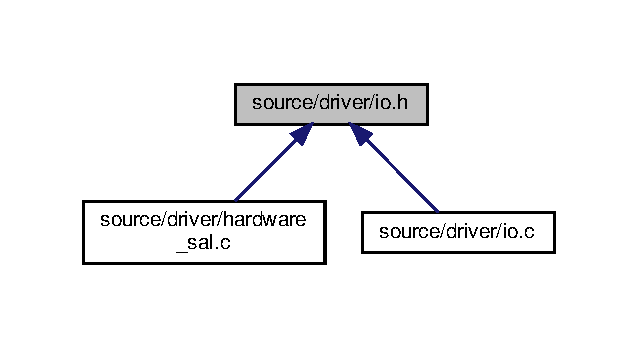
\includegraphics[width=306pt]{io_8h__dep__incl}
\end{center}
\end{figure}
\subsection*{Functions}
\begin{DoxyCompactItemize}
\item 
int \hyperlink{io_8h_a12ce98b64f2019ac45b44826a4db7ec9}{io\+\_\+init} ()
\begin{DoxyCompactList}\small\item\em Initialize lib\+Comedi in \char`\"{}\+Sanntidssalen\char`\"{}. \end{DoxyCompactList}\item 
void \hyperlink{io_8h_a43faae81f7fd5a3457a7cb86cd1010e2}{io\+\_\+set\+Bit} (int channel)
\begin{DoxyCompactList}\small\item\em Sets a digital channel bit. \end{DoxyCompactList}\item 
void \hyperlink{io_8h_a77b8ca35f291bea783684e3061abd7fe}{io\+\_\+clear\+Bit} (int channel)
\begin{DoxyCompactList}\small\item\em Clears a digital channel bit. \end{DoxyCompactList}\item 
void \hyperlink{io_8h_ac59309697150563a99604fea292f7d0e}{io\+\_\+write\+Analog} (int channel, int value)
\begin{DoxyCompactList}\small\item\em Writes a value to an analog channel. \end{DoxyCompactList}\item 
int \hyperlink{io_8h_a86b16b98f978fd95d983ebc57c022c3c}{io\+\_\+read\+Bit} (int channel)
\begin{DoxyCompactList}\small\item\em Reads a bit value from a digital channel. \end{DoxyCompactList}\item 
int \hyperlink{io_8h_aa01965057e77cb7406bd3dd3329fc230}{io\+\_\+read\+Analog} (int channel)
\begin{DoxyCompactList}\small\item\em Reads a bit value from an analog channel. \end{DoxyCompactList}\end{DoxyCompactItemize}


\subsection{Detailed Description}
Wrapper for lib\+Comedi I/O. These functions provide and interface to lib\+Comedi limited to use in the real time lab. 2006, Martin Korsgaard. 



\subsection{Function Documentation}
\mbox{\Hypertarget{io_8h_a77b8ca35f291bea783684e3061abd7fe}\label{io_8h_a77b8ca35f291bea783684e3061abd7fe}} 
\index{io.\+h@{io.\+h}!io\+\_\+clear\+Bit@{io\+\_\+clear\+Bit}}
\index{io\+\_\+clear\+Bit@{io\+\_\+clear\+Bit}!io.\+h@{io.\+h}}
\subsubsection{\texorpdfstring{io\+\_\+clear\+Bit()}{io\_clearBit()}}
{\footnotesize\ttfamily void io\+\_\+clear\+Bit (\begin{DoxyParamCaption}\item[{int}]{channel }\end{DoxyParamCaption})}



Clears a digital channel bit. 


\begin{DoxyParams}{Parameters}
{\em channel} & Channel bit to set. \\
\hline
\end{DoxyParams}


Definition at line 43 of file io.\+c.

\mbox{\Hypertarget{io_8h_a12ce98b64f2019ac45b44826a4db7ec9}\label{io_8h_a12ce98b64f2019ac45b44826a4db7ec9}} 
\index{io.\+h@{io.\+h}!io\+\_\+init@{io\+\_\+init}}
\index{io\+\_\+init@{io\+\_\+init}!io.\+h@{io.\+h}}
\subsubsection{\texorpdfstring{io\+\_\+init()}{io\_init()}}
{\footnotesize\ttfamily int io\+\_\+init (\begin{DoxyParamCaption}{ }\end{DoxyParamCaption})}



Initialize lib\+Comedi in \char`\"{}\+Sanntidssalen\char`\"{}. 

\begin{DoxyReturn}{Returns}
Non-\/zero on success and 0 on failure 
\end{DoxyReturn}


Definition at line 16 of file io.\+c.

\mbox{\Hypertarget{io_8h_aa01965057e77cb7406bd3dd3329fc230}\label{io_8h_aa01965057e77cb7406bd3dd3329fc230}} 
\index{io.\+h@{io.\+h}!io\+\_\+read\+Analog@{io\+\_\+read\+Analog}}
\index{io\+\_\+read\+Analog@{io\+\_\+read\+Analog}!io.\+h@{io.\+h}}
\subsubsection{\texorpdfstring{io\+\_\+read\+Analog()}{io\_readAnalog()}}
{\footnotesize\ttfamily int io\+\_\+read\+Analog (\begin{DoxyParamCaption}\item[{int}]{channel }\end{DoxyParamCaption})}



Reads a bit value from an analog channel. 


\begin{DoxyParams}{Parameters}
{\em channel} & Channel to read from. \\
\hline
\end{DoxyParams}
\begin{DoxyReturn}{Returns}
Value read. 
\end{DoxyReturn}


Definition at line 64 of file io.\+c.

\mbox{\Hypertarget{io_8h_a86b16b98f978fd95d983ebc57c022c3c}\label{io_8h_a86b16b98f978fd95d983ebc57c022c3c}} 
\index{io.\+h@{io.\+h}!io\+\_\+read\+Bit@{io\+\_\+read\+Bit}}
\index{io\+\_\+read\+Bit@{io\+\_\+read\+Bit}!io.\+h@{io.\+h}}
\subsubsection{\texorpdfstring{io\+\_\+read\+Bit()}{io\_readBit()}}
{\footnotesize\ttfamily int io\+\_\+read\+Bit (\begin{DoxyParamCaption}\item[{int}]{channel }\end{DoxyParamCaption})}



Reads a bit value from a digital channel. 


\begin{DoxyParams}{Parameters}
{\em channel} & Channel to read from. \\
\hline
\end{DoxyParams}
\begin{DoxyReturn}{Returns}
Value read. 
\end{DoxyReturn}


Definition at line 55 of file io.\+c.

\mbox{\Hypertarget{io_8h_a43faae81f7fd5a3457a7cb86cd1010e2}\label{io_8h_a43faae81f7fd5a3457a7cb86cd1010e2}} 
\index{io.\+h@{io.\+h}!io\+\_\+set\+Bit@{io\+\_\+set\+Bit}}
\index{io\+\_\+set\+Bit@{io\+\_\+set\+Bit}!io.\+h@{io.\+h}}
\subsubsection{\texorpdfstring{io\+\_\+set\+Bit()}{io\_setBit()}}
{\footnotesize\ttfamily void io\+\_\+set\+Bit (\begin{DoxyParamCaption}\item[{int}]{channel }\end{DoxyParamCaption})}



Sets a digital channel bit. 


\begin{DoxyParams}{Parameters}
{\em channel} & Channel bit to set. \\
\hline
\end{DoxyParams}


Definition at line 37 of file io.\+c.

\mbox{\Hypertarget{io_8h_ac59309697150563a99604fea292f7d0e}\label{io_8h_ac59309697150563a99604fea292f7d0e}} 
\index{io.\+h@{io.\+h}!io\+\_\+write\+Analog@{io\+\_\+write\+Analog}}
\index{io\+\_\+write\+Analog@{io\+\_\+write\+Analog}!io.\+h@{io.\+h}}
\subsubsection{\texorpdfstring{io\+\_\+write\+Analog()}{io\_writeAnalog()}}
{\footnotesize\ttfamily void io\+\_\+write\+Analog (\begin{DoxyParamCaption}\item[{int}]{channel,  }\item[{int}]{value }\end{DoxyParamCaption})}



Writes a value to an analog channel. 


\begin{DoxyParams}{Parameters}
{\em channel} & Channel to write to. \\
\hline
{\em value} & Value to write. \\
\hline
\end{DoxyParams}


Definition at line 49 of file io.\+c.


\hypertarget{hardware_8h}{}\section{source/hardware.h File Reference}
\label{hardware_8h}\index{source/hardware.\+h@{source/hardware.\+h}}


Driver for the elevator hardware.  


This graph shows which files directly or indirectly include this file\+:\nopagebreak
\begin{figure}[H]
\begin{center}
\leavevmode
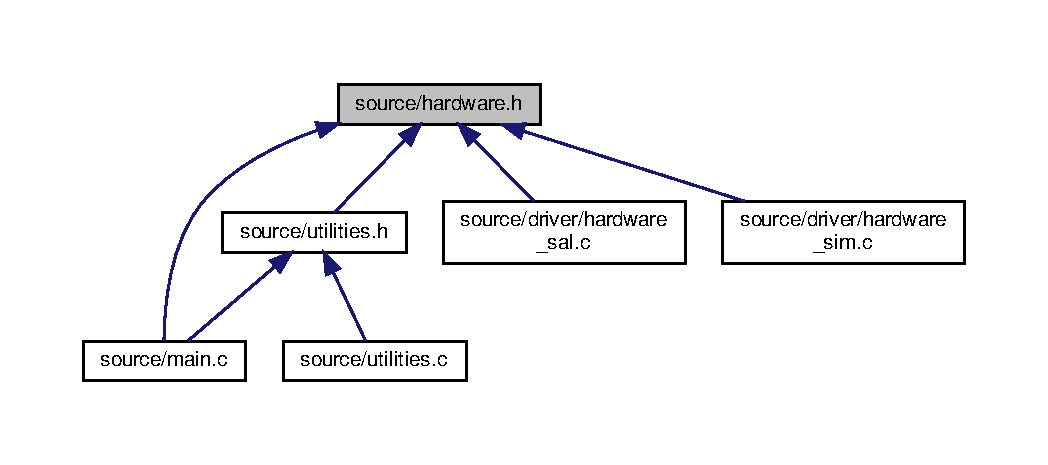
\includegraphics[width=350pt]{hardware_8h__dep__incl}
\end{center}
\end{figure}
\subsection*{Macros}
\begin{DoxyCompactItemize}
\item 
\mbox{\Hypertarget{hardware_8h_ae9e42615eade15633bd8c03b7a271a00}\label{hardware_8h_ae9e42615eade15633bd8c03b7a271a00}} 
\#define {\bfseries H\+A\+R\+D\+W\+A\+R\+E\+\_\+\+N\+U\+M\+B\+E\+R\+\_\+\+O\+F\+\_\+\+F\+L\+O\+O\+RS}~4
\item 
\mbox{\Hypertarget{hardware_8h_a966cbacea011640db5803364bff5ed53}\label{hardware_8h_a966cbacea011640db5803364bff5ed53}} 
\#define {\bfseries H\+A\+R\+D\+W\+A\+R\+E\+\_\+\+N\+U\+M\+B\+E\+R\+\_\+\+O\+F\+\_\+\+B\+U\+T\+T\+O\+NS}~3
\item 
\mbox{\Hypertarget{hardware_8h_a33ce204ffef85668d2ecffe042b5daab}\label{hardware_8h_a33ce204ffef85668d2ecffe042b5daab}} 
\#define {\bfseries H\+A\+R\+D\+W\+A\+R\+E\+\_\+\+W\+A\+I\+T\+I\+N\+G\+T\+I\+ME}~3
\item 
\mbox{\Hypertarget{hardware_8h_a6185c96166318ded1f458ece45e14726}\label{hardware_8h_a6185c96166318ded1f458ece45e14726}} 
\#define {\bfseries D\+I\+R\+E\+C\+T\+I\+O\+N\+\_\+\+UP}~0
\item 
\mbox{\Hypertarget{hardware_8h_a854f9aaf17c5861c78f3a35a1b4e2f74}\label{hardware_8h_a854f9aaf17c5861c78f3a35a1b4e2f74}} 
\#define {\bfseries D\+I\+R\+E\+C\+T\+I\+O\+N\+\_\+\+D\+O\+WN}~1
\end{DoxyCompactItemize}
\subsection*{Enumerations}
\begin{DoxyCompactItemize}
\item 
\mbox{\Hypertarget{hardware_8h_a2167c399a24df296afc432bcb88228af}\label{hardware_8h_a2167c399a24df296afc432bcb88228af}} 
enum \hyperlink{hardware_8h_a2167c399a24df296afc432bcb88228af}{Hardware\+Movement} \{ {\bfseries H\+A\+R\+D\+W\+A\+R\+E\+\_\+\+M\+O\+V\+E\+M\+E\+N\+T\+\_\+\+UP}, 
{\bfseries H\+A\+R\+D\+W\+A\+R\+E\+\_\+\+M\+O\+V\+E\+M\+E\+N\+T\+\_\+\+S\+T\+OP}, 
{\bfseries H\+A\+R\+D\+W\+A\+R\+E\+\_\+\+M\+O\+V\+E\+M\+E\+N\+T\+\_\+\+D\+O\+WN}
 \}\begin{DoxyCompactList}\small\item\em Movement type used in {\ttfamily hardware\+\_\+command\+Movement}. \end{DoxyCompactList}
\item 
\mbox{\Hypertarget{hardware_8h_a796a8de8ce0ae769d7dbd3327a7bdbe7}\label{hardware_8h_a796a8de8ce0ae769d7dbd3327a7bdbe7}} 
enum \hyperlink{hardware_8h_a796a8de8ce0ae769d7dbd3327a7bdbe7}{Hardware\+Order} \{ {\bfseries H\+A\+R\+D\+W\+A\+R\+E\+\_\+\+O\+R\+D\+E\+R\+\_\+\+UP}, 
{\bfseries H\+A\+R\+D\+W\+A\+R\+E\+\_\+\+O\+R\+D\+E\+R\+\_\+\+I\+N\+S\+I\+DE}, 
{\bfseries H\+A\+R\+D\+W\+A\+R\+E\+\_\+\+O\+R\+D\+E\+R\+\_\+\+D\+O\+WN}
 \}\begin{DoxyCompactList}\small\item\em Order type used in {\ttfamily hardware\+\_\+read\+Order} and in {\ttfamily hardware\+\_\+command\+Order\+Light}. \end{DoxyCompactList}
\end{DoxyCompactItemize}
\subsection*{Functions}
\begin{DoxyCompactItemize}
\item 
int \hyperlink{hardware_8h_a054b8fb8768311d46be58d6a4890d771}{hardware\+\_\+init} ()
\begin{DoxyCompactList}\small\item\em Initializes the elevator control hardware. Must be called once before other calls to the elevator hardware driver. \end{DoxyCompactList}\item 
void \hyperlink{hardware_8h_a2b26416f1ea2bfdfd9d4c70926357646}{hardware\+\_\+command\+Movement} (\hyperlink{hardware_8h_a2167c399a24df296afc432bcb88228af}{Hardware\+Movement} movement)
\begin{DoxyCompactList}\small\item\em Commands the elevator to either move up or down, or commands it to halt. \end{DoxyCompactList}\item 
int \hyperlink{hardware_8h_a765e0cb7413c766aa7271c3bb06728d7}{hardware\+\_\+read\+Stop\+Signal} ()
\begin{DoxyCompactList}\small\item\em Polls the hardware for the current stop signal. \end{DoxyCompactList}\item 
int \hyperlink{hardware_8h_ae592c4f3a5acff829bc734ab91a1b57f}{hardware\+\_\+read\+Obstruction\+Signal} ()
\begin{DoxyCompactList}\small\item\em Polls the hardware for the current obstruction signal. \end{DoxyCompactList}\item 
int \hyperlink{hardware_8h_a87d4d3ee2e6fe19bcb9c11e65fb92d53}{hardware\+\_\+read\+Floor\+Sensor} (int floor)
\begin{DoxyCompactList}\small\item\em Polls the floor sensor for the given {\ttfamily floor}. \end{DoxyCompactList}\item 
int \hyperlink{hardware_8h_abedc25428c63e1f5cc8e5dd14abee151}{hardware\+\_\+read\+Order} (int floor, \hyperlink{hardware_8h_a796a8de8ce0ae769d7dbd3327a7bdbe7}{Hardware\+Order} order\+\_\+type)
\begin{DoxyCompactList}\small\item\em Polls the hardware for the status of orders from floor {\ttfamily floor} of type {\ttfamily order\+\_\+type}. \end{DoxyCompactList}\item 
void \hyperlink{hardware_8h_ad27760d8ba208ba2b3666b7c90c62b39}{hardware\+\_\+command\+Door\+Open} (int door\+\_\+open)
\begin{DoxyCompactList}\small\item\em Commands the hardware to open-\/ or close the elevator door. \end{DoxyCompactList}\item 
void \hyperlink{hardware_8h_af5f675da2619585072fcdf690b67ea42}{hardware\+\_\+command\+Floor\+Indicator\+On} (int floor)
\begin{DoxyCompactList}\small\item\em Commands the hardware to turn on the floor indicator for {\ttfamily floor}. All indicators all mutually exclusive; other indicator lights will turn off. \end{DoxyCompactList}\item 
void \hyperlink{hardware_8h_a7249fcc1e3b3cde04c58306074fbfe01}{hardware\+\_\+command\+Stop\+Light} (int on)
\begin{DoxyCompactList}\small\item\em Sets the light in the panel stop button. \end{DoxyCompactList}\item 
void \hyperlink{hardware_8h_a3f3f545d0868c9770bb13df48a713c58}{hardware\+\_\+command\+Order\+Light} (int floor, \hyperlink{hardware_8h_a796a8de8ce0ae769d7dbd3327a7bdbe7}{Hardware\+Order} order\+\_\+type, int on)
\begin{DoxyCompactList}\small\item\em Sets the light in a button corresponding to an order of type {\ttfamily order\+\_\+type}, at floor {\ttfamily floor}. \end{DoxyCompactList}\end{DoxyCompactItemize}


\subsection{Detailed Description}
Driver for the elevator hardware. 



\subsection{Function Documentation}
\mbox{\Hypertarget{hardware_8h_ad27760d8ba208ba2b3666b7c90c62b39}\label{hardware_8h_ad27760d8ba208ba2b3666b7c90c62b39}} 
\index{hardware.\+h@{hardware.\+h}!hardware\+\_\+command\+Door\+Open@{hardware\+\_\+command\+Door\+Open}}
\index{hardware\+\_\+command\+Door\+Open@{hardware\+\_\+command\+Door\+Open}!hardware.\+h@{hardware.\+h}}
\subsubsection{\texorpdfstring{hardware\+\_\+command\+Door\+Open()}{hardware\_commandDoorOpen()}}
{\footnotesize\ttfamily void hardware\+\_\+command\+Door\+Open (\begin{DoxyParamCaption}\item[{int}]{door\+\_\+open }\end{DoxyParamCaption})}



Commands the hardware to open-\/ or close the elevator door. 


\begin{DoxyParams}{Parameters}
{\em door\+\_\+open} & A truthy value (non-\/zero) to open the door; 0 to close. \\
\hline
\end{DoxyParams}


Definition at line 138 of file hardware\+\_\+sal.\+c.

\mbox{\Hypertarget{hardware_8h_af5f675da2619585072fcdf690b67ea42}\label{hardware_8h_af5f675da2619585072fcdf690b67ea42}} 
\index{hardware.\+h@{hardware.\+h}!hardware\+\_\+command\+Floor\+Indicator\+On@{hardware\+\_\+command\+Floor\+Indicator\+On}}
\index{hardware\+\_\+command\+Floor\+Indicator\+On@{hardware\+\_\+command\+Floor\+Indicator\+On}!hardware.\+h@{hardware.\+h}}
\subsubsection{\texorpdfstring{hardware\+\_\+command\+Floor\+Indicator\+On()}{hardware\_commandFloorIndicatorOn()}}
{\footnotesize\ttfamily void hardware\+\_\+command\+Floor\+Indicator\+On (\begin{DoxyParamCaption}\item[{int}]{floor }\end{DoxyParamCaption})}



Commands the hardware to turn on the floor indicator for {\ttfamily floor}. All indicators all mutually exclusive; other indicator lights will turn off. 


\begin{DoxyParams}{Parameters}
{\em floor} & Floor to turn on the indicator for.\\
\hline
\end{DoxyParams}
\begin{DoxyWarning}{Warning}
Owing to peculiarities in the hardware construction, there will always be one indicator active. 
\end{DoxyWarning}


Definition at line 147 of file hardware\+\_\+sal.\+c.

\mbox{\Hypertarget{hardware_8h_a2b26416f1ea2bfdfd9d4c70926357646}\label{hardware_8h_a2b26416f1ea2bfdfd9d4c70926357646}} 
\index{hardware.\+h@{hardware.\+h}!hardware\+\_\+command\+Movement@{hardware\+\_\+command\+Movement}}
\index{hardware\+\_\+command\+Movement@{hardware\+\_\+command\+Movement}!hardware.\+h@{hardware.\+h}}
\subsubsection{\texorpdfstring{hardware\+\_\+command\+Movement()}{hardware\_commandMovement()}}
{\footnotesize\ttfamily void hardware\+\_\+command\+Movement (\begin{DoxyParamCaption}\item[{\hyperlink{hardware_8h_a2167c399a24df296afc432bcb88228af}{Hardware\+Movement}}]{movement }\end{DoxyParamCaption})}



Commands the elevator to either move up or down, or commands it to halt. 


\begin{DoxyParams}{Parameters}
{\em movement} & Commanded movement. \\
\hline
\end{DoxyParams}


Definition at line 69 of file hardware\+\_\+sal.\+c.

\mbox{\Hypertarget{hardware_8h_a3f3f545d0868c9770bb13df48a713c58}\label{hardware_8h_a3f3f545d0868c9770bb13df48a713c58}} 
\index{hardware.\+h@{hardware.\+h}!hardware\+\_\+command\+Order\+Light@{hardware\+\_\+command\+Order\+Light}}
\index{hardware\+\_\+command\+Order\+Light@{hardware\+\_\+command\+Order\+Light}!hardware.\+h@{hardware.\+h}}
\subsubsection{\texorpdfstring{hardware\+\_\+command\+Order\+Light()}{hardware\_commandOrderLight()}}
{\footnotesize\ttfamily void hardware\+\_\+command\+Order\+Light (\begin{DoxyParamCaption}\item[{int}]{floor,  }\item[{\hyperlink{hardware_8h_a796a8de8ce0ae769d7dbd3327a7bdbe7}{Hardware\+Order}}]{order\+\_\+type,  }\item[{int}]{on }\end{DoxyParamCaption})}



Sets the light in a button corresponding to an order of type {\ttfamily order\+\_\+type}, at floor {\ttfamily floor}. 


\begin{DoxyParams}{Parameters}
{\em floor} & The floor of the order indicator. \\
\hline
{\em order\+\_\+type} & The type of order. \\
\hline
{\em on} & A truthy value (non-\/zero) to turn the light on; 0 to turn it off. \\
\hline
\end{DoxyParams}


Definition at line 172 of file hardware\+\_\+sal.\+c.

\mbox{\Hypertarget{hardware_8h_a7249fcc1e3b3cde04c58306074fbfe01}\label{hardware_8h_a7249fcc1e3b3cde04c58306074fbfe01}} 
\index{hardware.\+h@{hardware.\+h}!hardware\+\_\+command\+Stop\+Light@{hardware\+\_\+command\+Stop\+Light}}
\index{hardware\+\_\+command\+Stop\+Light@{hardware\+\_\+command\+Stop\+Light}!hardware.\+h@{hardware.\+h}}
\subsubsection{\texorpdfstring{hardware\+\_\+command\+Stop\+Light()}{hardware\_commandStopLight()}}
{\footnotesize\ttfamily void hardware\+\_\+command\+Stop\+Light (\begin{DoxyParamCaption}\item[{int}]{on }\end{DoxyParamCaption})}



Sets the light in the panel stop button. 


\begin{DoxyParams}{Parameters}
{\em on} & A truthy value (non-\/zero) to turn the light on; 0 to turn it off. \\
\hline
\end{DoxyParams}


Definition at line 163 of file hardware\+\_\+sal.\+c.

\mbox{\Hypertarget{hardware_8h_a054b8fb8768311d46be58d6a4890d771}\label{hardware_8h_a054b8fb8768311d46be58d6a4890d771}} 
\index{hardware.\+h@{hardware.\+h}!hardware\+\_\+init@{hardware\+\_\+init}}
\index{hardware\+\_\+init@{hardware\+\_\+init}!hardware.\+h@{hardware.\+h}}
\subsubsection{\texorpdfstring{hardware\+\_\+init()}{hardware\_init()}}
{\footnotesize\ttfamily int hardware\+\_\+init (\begin{DoxyParamCaption}{ }\end{DoxyParamCaption})}



Initializes the elevator control hardware. Must be called once before other calls to the elevator hardware driver. 

\begin{DoxyReturn}{Returns}
0 on success. Non-\/zero for failure. 
\end{DoxyReturn}


Definition at line 45 of file hardware\+\_\+sal.\+c.

\mbox{\Hypertarget{hardware_8h_a87d4d3ee2e6fe19bcb9c11e65fb92d53}\label{hardware_8h_a87d4d3ee2e6fe19bcb9c11e65fb92d53}} 
\index{hardware.\+h@{hardware.\+h}!hardware\+\_\+read\+Floor\+Sensor@{hardware\+\_\+read\+Floor\+Sensor}}
\index{hardware\+\_\+read\+Floor\+Sensor@{hardware\+\_\+read\+Floor\+Sensor}!hardware.\+h@{hardware.\+h}}
\subsubsection{\texorpdfstring{hardware\+\_\+read\+Floor\+Sensor()}{hardware\_readFloorSensor()}}
{\footnotesize\ttfamily int hardware\+\_\+read\+Floor\+Sensor (\begin{DoxyParamCaption}\item[{int}]{floor }\end{DoxyParamCaption})}



Polls the floor sensor for the given {\ttfamily floor}. 


\begin{DoxyParams}{Parameters}
{\em floor} & Inquired floor.\\
\hline
\end{DoxyParams}
\begin{DoxyReturn}{Returns}
1 if the elevator is at {\ttfamily floor}, otherwise 0; 
\end{DoxyReturn}


Definition at line 95 of file hardware\+\_\+sal.\+c.

\mbox{\Hypertarget{hardware_8h_ae592c4f3a5acff829bc734ab91a1b57f}\label{hardware_8h_ae592c4f3a5acff829bc734ab91a1b57f}} 
\index{hardware.\+h@{hardware.\+h}!hardware\+\_\+read\+Obstruction\+Signal@{hardware\+\_\+read\+Obstruction\+Signal}}
\index{hardware\+\_\+read\+Obstruction\+Signal@{hardware\+\_\+read\+Obstruction\+Signal}!hardware.\+h@{hardware.\+h}}
\subsubsection{\texorpdfstring{hardware\+\_\+read\+Obstruction\+Signal()}{hardware\_readObstructionSignal()}}
{\footnotesize\ttfamily int hardware\+\_\+read\+Obstruction\+Signal (\begin{DoxyParamCaption}{ }\end{DoxyParamCaption})}



Polls the hardware for the current obstruction signal. 

\begin{DoxyReturn}{Returns}
1 if the obstruction signal is high; 0 if it is low. 
\end{DoxyReturn}


Definition at line 91 of file hardware\+\_\+sal.\+c.

\mbox{\Hypertarget{hardware_8h_abedc25428c63e1f5cc8e5dd14abee151}\label{hardware_8h_abedc25428c63e1f5cc8e5dd14abee151}} 
\index{hardware.\+h@{hardware.\+h}!hardware\+\_\+read\+Order@{hardware\+\_\+read\+Order}}
\index{hardware\+\_\+read\+Order@{hardware\+\_\+read\+Order}!hardware.\+h@{hardware.\+h}}
\subsubsection{\texorpdfstring{hardware\+\_\+read\+Order()}{hardware\_readOrder()}}
{\footnotesize\ttfamily int hardware\+\_\+read\+Order (\begin{DoxyParamCaption}\item[{int}]{floor,  }\item[{\hyperlink{hardware_8h_a796a8de8ce0ae769d7dbd3327a7bdbe7}{Hardware\+Order}}]{order\+\_\+type }\end{DoxyParamCaption})}



Polls the hardware for the status of orders from floor {\ttfamily floor} of type {\ttfamily order\+\_\+type}. 


\begin{DoxyParams}{Parameters}
{\em floor} & Inquired floor. \\
\hline
{\em order\+\_\+type} & \\
\hline
\end{DoxyParams}
\begin{DoxyReturn}{Returns}
1 if the combination of {\ttfamily floor} and {\ttfamily order\+\_\+type} is being requested, otherwise 0. 
\end{DoxyReturn}


Definition at line 121 of file hardware\+\_\+sal.\+c.

\mbox{\Hypertarget{hardware_8h_a765e0cb7413c766aa7271c3bb06728d7}\label{hardware_8h_a765e0cb7413c766aa7271c3bb06728d7}} 
\index{hardware.\+h@{hardware.\+h}!hardware\+\_\+read\+Stop\+Signal@{hardware\+\_\+read\+Stop\+Signal}}
\index{hardware\+\_\+read\+Stop\+Signal@{hardware\+\_\+read\+Stop\+Signal}!hardware.\+h@{hardware.\+h}}
\subsubsection{\texorpdfstring{hardware\+\_\+read\+Stop\+Signal()}{hardware\_readStopSignal()}}
{\footnotesize\ttfamily int hardware\+\_\+read\+Stop\+Signal (\begin{DoxyParamCaption}{ }\end{DoxyParamCaption})}



Polls the hardware for the current stop signal. 

\begin{DoxyReturn}{Returns}
1 if the stop signal is high; 0 if it is low. 
\end{DoxyReturn}


Definition at line 87 of file hardware\+\_\+sal.\+c.


\hypertarget{state_8h}{}\section{source/state.h File Reference}
\label{state_8h}\index{source/state.\+h@{source/state.\+h}}


States for the finite state machine.  


{\ttfamily \#include $<$time.\+h$>$}\newline
Include dependency graph for state.\+h\+:\nopagebreak
\begin{figure}[H]
\begin{center}
\leavevmode
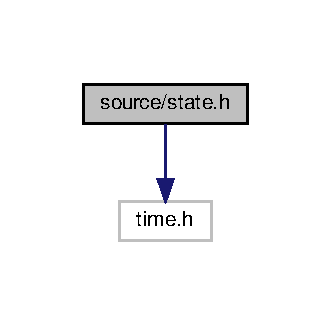
\includegraphics[width=159pt]{state_8h__incl}
\end{center}
\end{figure}
This graph shows which files directly or indirectly include this file\+:\nopagebreak
\begin{figure}[H]
\begin{center}
\leavevmode
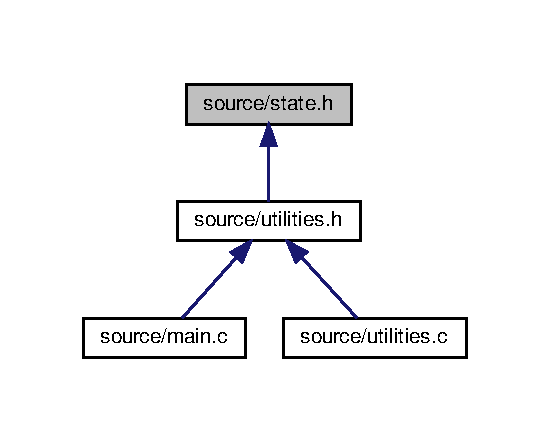
\includegraphics[width=264pt]{state_8h__dep__incl}
\end{center}
\end{figure}
\subsection*{Data Structures}
\begin{DoxyCompactItemize}
\item 
struct \hyperlink{structState}{State}
\begin{DoxyCompactList}\small\item\em A struct with members that hold information about the elevators state. \end{DoxyCompactList}\end{DoxyCompactItemize}


\subsection{Detailed Description}
States for the finite state machine. 


\hypertarget{utilities_8h}{}\section{source/utilities.h File Reference}
\label{utilities_8h}\index{source/utilities.\+h@{source/utilities.\+h}}


Utility-\/functions that is used to make decisions regarding the initialization and handling of the fsm, as well as the high level logic of the hardware.  


{\ttfamily \#include $<$stdio.\+h$>$}\newline
{\ttfamily \#include $<$stdlib.\+h$>$}\newline
{\ttfamily \#include $<$signal.\+h$>$}\newline
{\ttfamily \#include \char`\"{}hardware.\+h\char`\"{}}\newline
{\ttfamily \#include \char`\"{}state.\+h\char`\"{}}\newline
Include dependency graph for utilities.\+h\+:\nopagebreak
\begin{figure}[H]
\begin{center}
\leavevmode
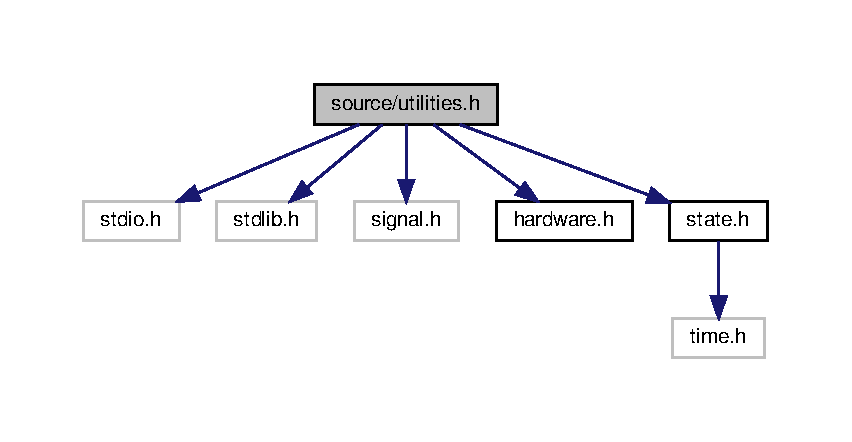
\includegraphics[width=350pt]{utilities_8h__incl}
\end{center}
\end{figure}
This graph shows which files directly or indirectly include this file\+:\nopagebreak
\begin{figure}[H]
\begin{center}
\leavevmode
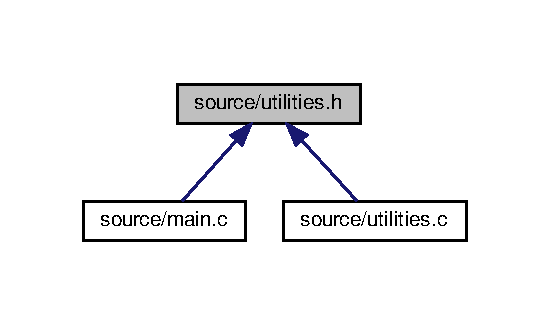
\includegraphics[width=264pt]{utilities_8h__dep__incl}
\end{center}
\end{figure}
\subsection*{Functions}
\begin{DoxyCompactItemize}
\item 
int \hyperlink{utilities_8h_ad23a19d30fe8a79d4d57ef7cf1b27606}{orders\+\_\+scan\+Up} (struct \hyperlink{structState}{State} $\ast$current\+State)
\begin{DoxyCompactList}\small\item\em Searches through all orders above the last floor visited. \end{DoxyCompactList}\item 
int \hyperlink{utilities_8h_a1e5ed8d6b7162e8a6108c26bb95f90c3}{orders\+\_\+scan\+Down} (struct \hyperlink{structState}{State} $\ast$current\+State)
\begin{DoxyCompactList}\small\item\em Searches through all orders under the last floor visited. \end{DoxyCompactList}\item 
int \hyperlink{utilities_8h_a2d994e25f4eb46c506ea09ab19903091}{orders\+\_\+is\+Empty} (struct \hyperlink{structState}{State} $\ast$current\+State)
\begin{DoxyCompactList}\small\item\em Searches for true elements in the orderbook of the {\ttfamily current\+State}. \end{DoxyCompactList}\item 
void \hyperlink{utilities_8h_aa24ca3fc02bc1ae9fa9fdcbd3676643b}{orders\+\_\+reset} (struct \hyperlink{structState}{State} $\ast$current\+State)
\begin{DoxyCompactList}\small\item\em Resets all elements in the orderbook of the {\ttfamily current\+State}. \end{DoxyCompactList}\item 
void \hyperlink{utilities_8h_afed71a3659d78a493d5a26711c8f2c90}{orders\+\_\+update} (struct \hyperlink{structState}{State} $\ast$current\+State)
\begin{DoxyCompactList}\small\item\em Checks if any of the order buttons is pressed and sets the corresponding element in the orderbook of the {\ttfamily current\+State} to 1. \end{DoxyCompactList}\item 
void \hyperlink{utilities_8h_aa61b141d1f8439848f30338ea8020420}{orders\+\_\+check\+Peripherals} (struct \hyperlink{structState}{State} $\ast$current\+State)
\begin{DoxyCompactList}\small\item\em Checks for additional orders in the direction of the {\ttfamily current\+State} . If there is no more orders in the peripheral and the door is closed, the direction of the {\ttfamily current\+State} is flipped. If there is an active order in the current floor heading in the new direction, the routine\+\_\+arrival function is called. \end{DoxyCompactList}\item 
void \hyperlink{utilities_8h_ab40428b043fc935b46473809a2713526}{routine\+\_\+start\+Motor} (struct \hyperlink{structState}{State} $\ast$current\+State)
\begin{DoxyCompactList}\small\item\em Starts the motor in the direction of the {\ttfamily current\+State} provided that the door is closed and that there exists an order. \end{DoxyCompactList}\item 
void \hyperlink{utilities_8h_aa99be307bbfe1745a10b5f93b549d604}{routine\+\_\+stop} (struct \hyperlink{structState}{State} $\ast$current\+State)
\begin{DoxyCompactList}\small\item\em Excecutes the routine associated with the stop-\/button being pressed. This involves\+: Resetting the orderbook and all order lights Setting fsm\+\_\+stop of the {\ttfamily current\+State} to 1 Halting the elevator Opening the doors if the elevator is at a defined floor. \end{DoxyCompactList}\item 
void \hyperlink{utilities_8h_ac1169440a22b18c47a59eb919b6b5793}{routine\+\_\+arrival} (struct \hyperlink{structState}{State} $\ast$current\+State)
\begin{DoxyCompactList}\small\item\em Excecutes the routine associated with the elevator halting at a floor. This involves\+: Halting the elevator Opening the door Resetting the orders and order lights on the current floor. \end{DoxyCompactList}\item 
void \hyperlink{utilities_8h_afa402716aa64282819669dbfe0df67c2}{initialize\+\_\+hardware} ()
\begin{DoxyCompactList}\small\item\em Resets all lights realated to the elevator and initializes the input/output ports. \end{DoxyCompactList}\item 
void \hyperlink{utilities_8h_a3e2cbb6422ab3aba897afa93806356f4}{initialize\+\_\+state} (struct \hyperlink{structState}{State} $\ast$current\+State)
\begin{DoxyCompactList}\small\item\em Sets all values of {\ttfamily current\+State} to the preferred initial values. This involves\+: Setting fsm\+\_\+floor to the top floor Setting the fsm\+\_\+ignore\+All\+Orders of the {\ttfamily current\+State} and setting an order in the first floor, which will send the elevator to the first floor Resetting fsm\+\_\+stop, fsm\+\_\+door and timer\+\_\+start\+Time Setting fsm\+\_\+direction to down. \end{DoxyCompactList}\item 
\mbox{\Hypertarget{utilities_8h_aa6aac2968b7f6a8c55b257c9c4371b9e}\label{utilities_8h_aa6aac2968b7f6a8c55b257c9c4371b9e}} 
void \hyperlink{utilities_8h_aa6aac2968b7f6a8c55b257c9c4371b9e}{initialize\+\_\+clear\+All\+Order\+Lights} ()
\begin{DoxyCompactList}\small\item\em Resets all lights related to the elevator. \end{DoxyCompactList}\item 
void \hyperlink{utilities_8h_ae51781081a78a682f050b705cad4e23a}{handler\+\_\+close\+Door} (struct \hyperlink{structState}{State} $\ast$current\+State)
\begin{DoxyCompactList}\small\item\em Closes the doors and turns off the door-\/light if the doors have been open for more than the timer\+\_\+waiting\+Time of the {\ttfamily current\+State}. \end{DoxyCompactList}\item 
void \hyperlink{utilities_8h_a5ee8a7ab22d1b1e8611ebb6981a278f3}{handler\+\_\+keep\+Door\+Open} (struct \hyperlink{structState}{State} $\ast$current\+State)
\begin{DoxyCompactList}\small\item\em Restarts the door-\/timer of the {\ttfamily current\+State} if the obstruction signal or stop button is active while the doors are open. \end{DoxyCompactList}\item 
void \hyperlink{utilities_8h_a54fab6fc7214ab25199b43f69ea0b479}{handler\+\_\+first\+Order\+After\+Stop} (struct \hyperlink{structState}{State} $\ast$current\+State)
\begin{DoxyCompactList}\small\item\em Handles the special case when the first order after a stop-\/state is recieved This requires extra logic because the elevator might be between floors. \end{DoxyCompactList}\item 
void \hyperlink{utilities_8h_a270694feded09657dfd08d9199c433d5}{handler\+\_\+floor\+Sensors} (struct \hyperlink{structState}{State} $\ast$current\+State)
\begin{DoxyCompactList}\small\item\em If there is an active floor sensor, the function check\+\_\+halt is called to decide whether or not to take a halt. If so, the halt is excecuted. The floor light of the active floor will be set. \end{DoxyCompactList}\item 
int \hyperlink{utilities_8h_a9d5d7d239279fcd60789ef49b1f02e48}{check\+\_\+halt} (struct \hyperlink{structState}{State} $\ast$current\+State)
\begin{DoxyCompactList}\small\item\em Compares the current floor, the current direction and the orderbook of the {\ttfamily current\+State} to decide whether or not the elevator should take a halt. \end{DoxyCompactList}\end{DoxyCompactItemize}


\subsection{Detailed Description}
Utility-\/functions that is used to make decisions regarding the initialization and handling of the fsm, as well as the high level logic of the hardware. 



\subsection{Function Documentation}
\mbox{\Hypertarget{utilities_8h_a9d5d7d239279fcd60789ef49b1f02e48}\label{utilities_8h_a9d5d7d239279fcd60789ef49b1f02e48}} 
\index{utilities.\+h@{utilities.\+h}!check\+\_\+halt@{check\+\_\+halt}}
\index{check\+\_\+halt@{check\+\_\+halt}!utilities.\+h@{utilities.\+h}}
\subsubsection{\texorpdfstring{check\+\_\+halt()}{check\_halt()}}
{\footnotesize\ttfamily int check\+\_\+halt (\begin{DoxyParamCaption}\item[{struct \hyperlink{structState}{State} $\ast$}]{current\+State }\end{DoxyParamCaption})}



Compares the current floor, the current direction and the orderbook of the {\ttfamily current\+State} to decide whether or not the elevator should take a halt. 


\begin{DoxyParams}{Parameters}
{\em current\+State} & pointer to the current state of the elevator\\
\hline
\end{DoxyParams}
\begin{DoxyReturn}{Returns}
true if the elevator should take a halt, false if not 
\end{DoxyReturn}


Definition at line 243 of file utilities.\+c.

\mbox{\Hypertarget{utilities_8h_ae51781081a78a682f050b705cad4e23a}\label{utilities_8h_ae51781081a78a682f050b705cad4e23a}} 
\index{utilities.\+h@{utilities.\+h}!handler\+\_\+close\+Door@{handler\+\_\+close\+Door}}
\index{handler\+\_\+close\+Door@{handler\+\_\+close\+Door}!utilities.\+h@{utilities.\+h}}
\subsubsection{\texorpdfstring{handler\+\_\+close\+Door()}{handler\_closeDoor()}}
{\footnotesize\ttfamily void handler\+\_\+close\+Door (\begin{DoxyParamCaption}\item[{struct \hyperlink{structState}{State} $\ast$}]{current\+State }\end{DoxyParamCaption})}



Closes the doors and turns off the door-\/light if the doors have been open for more than the timer\+\_\+waiting\+Time of the {\ttfamily current\+State}. 


\begin{DoxyParams}{Parameters}
{\em current\+State} & pointer to the current state of the elevator \\
\hline
\end{DoxyParams}


Definition at line 132 of file utilities.\+c.

\mbox{\Hypertarget{utilities_8h_a54fab6fc7214ab25199b43f69ea0b479}\label{utilities_8h_a54fab6fc7214ab25199b43f69ea0b479}} 
\index{utilities.\+h@{utilities.\+h}!handler\+\_\+first\+Order\+After\+Stop@{handler\+\_\+first\+Order\+After\+Stop}}
\index{handler\+\_\+first\+Order\+After\+Stop@{handler\+\_\+first\+Order\+After\+Stop}!utilities.\+h@{utilities.\+h}}
\subsubsection{\texorpdfstring{handler\+\_\+first\+Order\+After\+Stop()}{handler\_firstOrderAfterStop()}}
{\footnotesize\ttfamily void handler\+\_\+first\+Order\+After\+Stop (\begin{DoxyParamCaption}\item[{struct \hyperlink{structState}{State} $\ast$}]{current\+State }\end{DoxyParamCaption})}



Handles the special case when the first order after a stop-\/state is recieved This requires extra logic because the elevator might be between floors. 


\begin{DoxyParams}{Parameters}
{\em current\+State} & pointer to the current state of the elevator\\
\hline
\end{DoxyParams}
\begin{DoxyWarning}{Warning}
The fsm\+\_\+floor of the {\ttfamily current\+State} might be manipulated in order to prevent bugs in the system 
\end{DoxyWarning}


Definition at line 140 of file utilities.\+c.

\mbox{\Hypertarget{utilities_8h_a270694feded09657dfd08d9199c433d5}\label{utilities_8h_a270694feded09657dfd08d9199c433d5}} 
\index{utilities.\+h@{utilities.\+h}!handler\+\_\+floor\+Sensors@{handler\+\_\+floor\+Sensors}}
\index{handler\+\_\+floor\+Sensors@{handler\+\_\+floor\+Sensors}!utilities.\+h@{utilities.\+h}}
\subsubsection{\texorpdfstring{handler\+\_\+floor\+Sensors()}{handler\_floorSensors()}}
{\footnotesize\ttfamily void handler\+\_\+floor\+Sensors (\begin{DoxyParamCaption}\item[{struct \hyperlink{structState}{State} $\ast$}]{current\+State }\end{DoxyParamCaption})}



If there is an active floor sensor, the function check\+\_\+halt is called to decide whether or not to take a halt. If so, the halt is excecuted. The floor light of the active floor will be set. 


\begin{DoxyParams}{Parameters}
{\em current\+State} & pointer to the current state of the elevator \\
\hline
\end{DoxyParams}


Definition at line 162 of file utilities.\+c.

\mbox{\Hypertarget{utilities_8h_a5ee8a7ab22d1b1e8611ebb6981a278f3}\label{utilities_8h_a5ee8a7ab22d1b1e8611ebb6981a278f3}} 
\index{utilities.\+h@{utilities.\+h}!handler\+\_\+keep\+Door\+Open@{handler\+\_\+keep\+Door\+Open}}
\index{handler\+\_\+keep\+Door\+Open@{handler\+\_\+keep\+Door\+Open}!utilities.\+h@{utilities.\+h}}
\subsubsection{\texorpdfstring{handler\+\_\+keep\+Door\+Open()}{handler\_keepDoorOpen()}}
{\footnotesize\ttfamily void handler\+\_\+keep\+Door\+Open (\begin{DoxyParamCaption}\item[{struct \hyperlink{structState}{State} $\ast$}]{current\+State }\end{DoxyParamCaption})}



Restarts the door-\/timer of the {\ttfamily current\+State} if the obstruction signal or stop button is active while the doors are open. 


\begin{DoxyParams}{Parameters}
{\em current\+State} & pointer to the current state of the elevator \\
\hline
\end{DoxyParams}


Definition at line 195 of file utilities.\+c.

\mbox{\Hypertarget{utilities_8h_afa402716aa64282819669dbfe0df67c2}\label{utilities_8h_afa402716aa64282819669dbfe0df67c2}} 
\index{utilities.\+h@{utilities.\+h}!initialize\+\_\+hardware@{initialize\+\_\+hardware}}
\index{initialize\+\_\+hardware@{initialize\+\_\+hardware}!utilities.\+h@{utilities.\+h}}
\subsubsection{\texorpdfstring{initialize\+\_\+hardware()}{initialize\_hardware()}}
{\footnotesize\ttfamily void initialize\+\_\+hardware (\begin{DoxyParamCaption}{ }\end{DoxyParamCaption})}



Resets all lights realated to the elevator and initializes the input/output ports. 

\begin{DoxyWarning}{Warning}
Will exit if the initialization of the input/ouput ports fails 
\end{DoxyWarning}


Definition at line 234 of file utilities.\+c.

\mbox{\Hypertarget{utilities_8h_a3e2cbb6422ab3aba897afa93806356f4}\label{utilities_8h_a3e2cbb6422ab3aba897afa93806356f4}} 
\index{utilities.\+h@{utilities.\+h}!initialize\+\_\+state@{initialize\+\_\+state}}
\index{initialize\+\_\+state@{initialize\+\_\+state}!utilities.\+h@{utilities.\+h}}
\subsubsection{\texorpdfstring{initialize\+\_\+state()}{initialize\_state()}}
{\footnotesize\ttfamily void initialize\+\_\+state (\begin{DoxyParamCaption}\item[{struct \hyperlink{structState}{State} $\ast$}]{current\+State }\end{DoxyParamCaption})}



Sets all values of {\ttfamily current\+State} to the preferred initial values. This involves\+: Setting fsm\+\_\+floor to the top floor Setting the fsm\+\_\+ignore\+All\+Orders of the {\ttfamily current\+State} and setting an order in the first floor, which will send the elevator to the first floor Resetting fsm\+\_\+stop, fsm\+\_\+door and timer\+\_\+start\+Time Setting fsm\+\_\+direction to down. 


\begin{DoxyParams}{Parameters}
{\em current\+State} & pointer to the current state of the elevator \\
\hline
\end{DoxyParams}


Definition at line 220 of file utilities.\+c.

\mbox{\Hypertarget{utilities_8h_aa61b141d1f8439848f30338ea8020420}\label{utilities_8h_aa61b141d1f8439848f30338ea8020420}} 
\index{utilities.\+h@{utilities.\+h}!orders\+\_\+check\+Peripherals@{orders\+\_\+check\+Peripherals}}
\index{orders\+\_\+check\+Peripherals@{orders\+\_\+check\+Peripherals}!utilities.\+h@{utilities.\+h}}
\subsubsection{\texorpdfstring{orders\+\_\+check\+Peripherals()}{orders\_checkPeripherals()}}
{\footnotesize\ttfamily void orders\+\_\+check\+Peripherals (\begin{DoxyParamCaption}\item[{struct \hyperlink{structState}{State} $\ast$}]{current\+State }\end{DoxyParamCaption})}



Checks for additional orders in the direction of the {\ttfamily current\+State} . If there is no more orders in the peripheral and the door is closed, the direction of the {\ttfamily current\+State} is flipped. If there is an active order in the current floor heading in the new direction, the routine\+\_\+arrival function is called. 


\begin{DoxyParams}{Parameters}
{\em current\+State} & pointer to the current state of the elevator \\
\hline
\end{DoxyParams}


Definition at line 64 of file utilities.\+c.

\mbox{\Hypertarget{utilities_8h_a2d994e25f4eb46c506ea09ab19903091}\label{utilities_8h_a2d994e25f4eb46c506ea09ab19903091}} 
\index{utilities.\+h@{utilities.\+h}!orders\+\_\+is\+Empty@{orders\+\_\+is\+Empty}}
\index{orders\+\_\+is\+Empty@{orders\+\_\+is\+Empty}!utilities.\+h@{utilities.\+h}}
\subsubsection{\texorpdfstring{orders\+\_\+is\+Empty()}{orders\_isEmpty()}}
{\footnotesize\ttfamily int orders\+\_\+is\+Empty (\begin{DoxyParamCaption}\item[{struct \hyperlink{structState}{State} $\ast$}]{current\+State }\end{DoxyParamCaption})}



Searches for true elements in the orderbook of the {\ttfamily current\+State}. 


\begin{DoxyParams}{Parameters}
{\em current\+State} & pointer to the current state of the elevator\\
\hline
\end{DoxyParams}
\begin{DoxyReturn}{Returns}
true if the orderbook is empty 
\end{DoxyReturn}


Definition at line 23 of file utilities.\+c.

\mbox{\Hypertarget{utilities_8h_aa24ca3fc02bc1ae9fa9fdcbd3676643b}\label{utilities_8h_aa24ca3fc02bc1ae9fa9fdcbd3676643b}} 
\index{utilities.\+h@{utilities.\+h}!orders\+\_\+reset@{orders\+\_\+reset}}
\index{orders\+\_\+reset@{orders\+\_\+reset}!utilities.\+h@{utilities.\+h}}
\subsubsection{\texorpdfstring{orders\+\_\+reset()}{orders\_reset()}}
{\footnotesize\ttfamily void orders\+\_\+reset (\begin{DoxyParamCaption}\item[{struct \hyperlink{structState}{State} $\ast$}]{current\+State }\end{DoxyParamCaption})}



Resets all elements in the orderbook of the {\ttfamily current\+State}. 


\begin{DoxyParams}{Parameters}
{\em current\+State} & pointer to the current state of the elevator \\
\hline
\end{DoxyParams}


Definition at line 31 of file utilities.\+c.

\mbox{\Hypertarget{utilities_8h_a1e5ed8d6b7162e8a6108c26bb95f90c3}\label{utilities_8h_a1e5ed8d6b7162e8a6108c26bb95f90c3}} 
\index{utilities.\+h@{utilities.\+h}!orders\+\_\+scan\+Down@{orders\+\_\+scan\+Down}}
\index{orders\+\_\+scan\+Down@{orders\+\_\+scan\+Down}!utilities.\+h@{utilities.\+h}}
\subsubsection{\texorpdfstring{orders\+\_\+scan\+Down()}{orders\_scanDown()}}
{\footnotesize\ttfamily int orders\+\_\+scan\+Down (\begin{DoxyParamCaption}\item[{struct \hyperlink{structState}{State} $\ast$}]{current\+State }\end{DoxyParamCaption})}



Searches through all orders under the last floor visited. 


\begin{DoxyParams}{Parameters}
{\em current\+State} & pointer to the current state of the elevator\\
\hline
\end{DoxyParams}
\begin{DoxyReturn}{Returns}
true if there exists an order under the current floor 
\end{DoxyReturn}


Definition at line 14 of file utilities.\+c.

\mbox{\Hypertarget{utilities_8h_ad23a19d30fe8a79d4d57ef7cf1b27606}\label{utilities_8h_ad23a19d30fe8a79d4d57ef7cf1b27606}} 
\index{utilities.\+h@{utilities.\+h}!orders\+\_\+scan\+Up@{orders\+\_\+scan\+Up}}
\index{orders\+\_\+scan\+Up@{orders\+\_\+scan\+Up}!utilities.\+h@{utilities.\+h}}
\subsubsection{\texorpdfstring{orders\+\_\+scan\+Up()}{orders\_scanUp()}}
{\footnotesize\ttfamily int orders\+\_\+scan\+Up (\begin{DoxyParamCaption}\item[{struct \hyperlink{structState}{State} $\ast$}]{current\+State }\end{DoxyParamCaption})}



Searches through all orders above the last floor visited. 


\begin{DoxyParams}{Parameters}
{\em current\+State} & pointer to the current state of the elevator\\
\hline
\end{DoxyParams}
\begin{DoxyReturn}{Returns}
true if there exists an order above the current floor 
\end{DoxyReturn}


Definition at line 4 of file utilities.\+c.

\mbox{\Hypertarget{utilities_8h_afed71a3659d78a493d5a26711c8f2c90}\label{utilities_8h_afed71a3659d78a493d5a26711c8f2c90}} 
\index{utilities.\+h@{utilities.\+h}!orders\+\_\+update@{orders\+\_\+update}}
\index{orders\+\_\+update@{orders\+\_\+update}!utilities.\+h@{utilities.\+h}}
\subsubsection{\texorpdfstring{orders\+\_\+update()}{orders\_update()}}
{\footnotesize\ttfamily void orders\+\_\+update (\begin{DoxyParamCaption}\item[{struct \hyperlink{structState}{State} $\ast$}]{current\+State }\end{DoxyParamCaption})}



Checks if any of the order buttons is pressed and sets the corresponding element in the orderbook of the {\ttfamily current\+State} to 1. 


\begin{DoxyParams}{Parameters}
{\em current\+State} & pointer to the current state of the elevator \\
\hline
\end{DoxyParams}


Definition at line 41 of file utilities.\+c.

\mbox{\Hypertarget{utilities_8h_ac1169440a22b18c47a59eb919b6b5793}\label{utilities_8h_ac1169440a22b18c47a59eb919b6b5793}} 
\index{utilities.\+h@{utilities.\+h}!routine\+\_\+arrival@{routine\+\_\+arrival}}
\index{routine\+\_\+arrival@{routine\+\_\+arrival}!utilities.\+h@{utilities.\+h}}
\subsubsection{\texorpdfstring{routine\+\_\+arrival()}{routine\_arrival()}}
{\footnotesize\ttfamily void routine\+\_\+arrival (\begin{DoxyParamCaption}\item[{struct \hyperlink{structState}{State} $\ast$}]{current\+State }\end{DoxyParamCaption})}



Excecutes the routine associated with the elevator halting at a floor. This involves\+: Halting the elevator Opening the door Resetting the orders and order lights on the current floor. 


\begin{DoxyParams}{Parameters}
{\em current\+State} & pointer to the current state of the elevator \\
\hline
\end{DoxyParams}


Definition at line 106 of file utilities.\+c.

\mbox{\Hypertarget{utilities_8h_ab40428b043fc935b46473809a2713526}\label{utilities_8h_ab40428b043fc935b46473809a2713526}} 
\index{utilities.\+h@{utilities.\+h}!routine\+\_\+start\+Motor@{routine\+\_\+start\+Motor}}
\index{routine\+\_\+start\+Motor@{routine\+\_\+start\+Motor}!utilities.\+h@{utilities.\+h}}
\subsubsection{\texorpdfstring{routine\+\_\+start\+Motor()}{routine\_startMotor()}}
{\footnotesize\ttfamily void routine\+\_\+start\+Motor (\begin{DoxyParamCaption}\item[{struct \hyperlink{structState}{State} $\ast$}]{current\+State }\end{DoxyParamCaption})}



Starts the motor in the direction of the {\ttfamily current\+State} provided that the door is closed and that there exists an order. 


\begin{DoxyParams}{Parameters}
{\em current\+State} & pointer to the current state of the elevator \\
\hline
\end{DoxyParams}


Definition at line 121 of file utilities.\+c.

\mbox{\Hypertarget{utilities_8h_aa99be307bbfe1745a10b5f93b549d604}\label{utilities_8h_aa99be307bbfe1745a10b5f93b549d604}} 
\index{utilities.\+h@{utilities.\+h}!routine\+\_\+stop@{routine\+\_\+stop}}
\index{routine\+\_\+stop@{routine\+\_\+stop}!utilities.\+h@{utilities.\+h}}
\subsubsection{\texorpdfstring{routine\+\_\+stop()}{routine\_stop()}}
{\footnotesize\ttfamily void routine\+\_\+stop (\begin{DoxyParamCaption}\item[{struct \hyperlink{structState}{State} $\ast$}]{current\+State }\end{DoxyParamCaption})}



Excecutes the routine associated with the stop-\/button being pressed. This involves\+: Resetting the orderbook and all order lights Setting fsm\+\_\+stop of the {\ttfamily current\+State} to 1 Halting the elevator Opening the doors if the elevator is at a defined floor. 


\begin{DoxyParams}{Parameters}
{\em current\+State} & pointer to the current state of the elevator \\
\hline
\end{DoxyParams}


Definition at line 90 of file utilities.\+c.


%--- End generated contents ---

% Index
\backmatter
\newpage
\phantomsection
\clearemptydoublepage
\addcontentsline{toc}{chapter}{Index}
\printindex

\end{document}
